\section*{Задача 6.1}
\subsection*{Постановка задачи}
Исследовать поведение погрешностей при численном дифференцировании функции.
\[
\begin{array}{| c | c | c |}
	\hline
	№ & f(x) & [a, b] \\ \hline
	5.2.52 & 6e^{-x}\sin{2\pi x} & [0, 3] \\ \hline
\end{array}
\]
\subsection*{Решение}
Для вычисления производной в точке $c = 0.9$ будем использовать 2 формулы - правой и левой разностной производной:
\begin{gather}
	f'(x) \approx \dfrac{f(c + h_k) - f(c)}{h_k}\\
	f'(x) \approx \dfrac{f(c) - f(c - h_k)}{h_k}
\end{gather}

Приведем графики погрешностей вычисления производных 1-го и 2-го порядка в точке $c = 0.9$.

\begin{figure}[h!]
	\centering                                                                                            
	\begin{minipage}{0.45\textwidth}
	        \centering
	        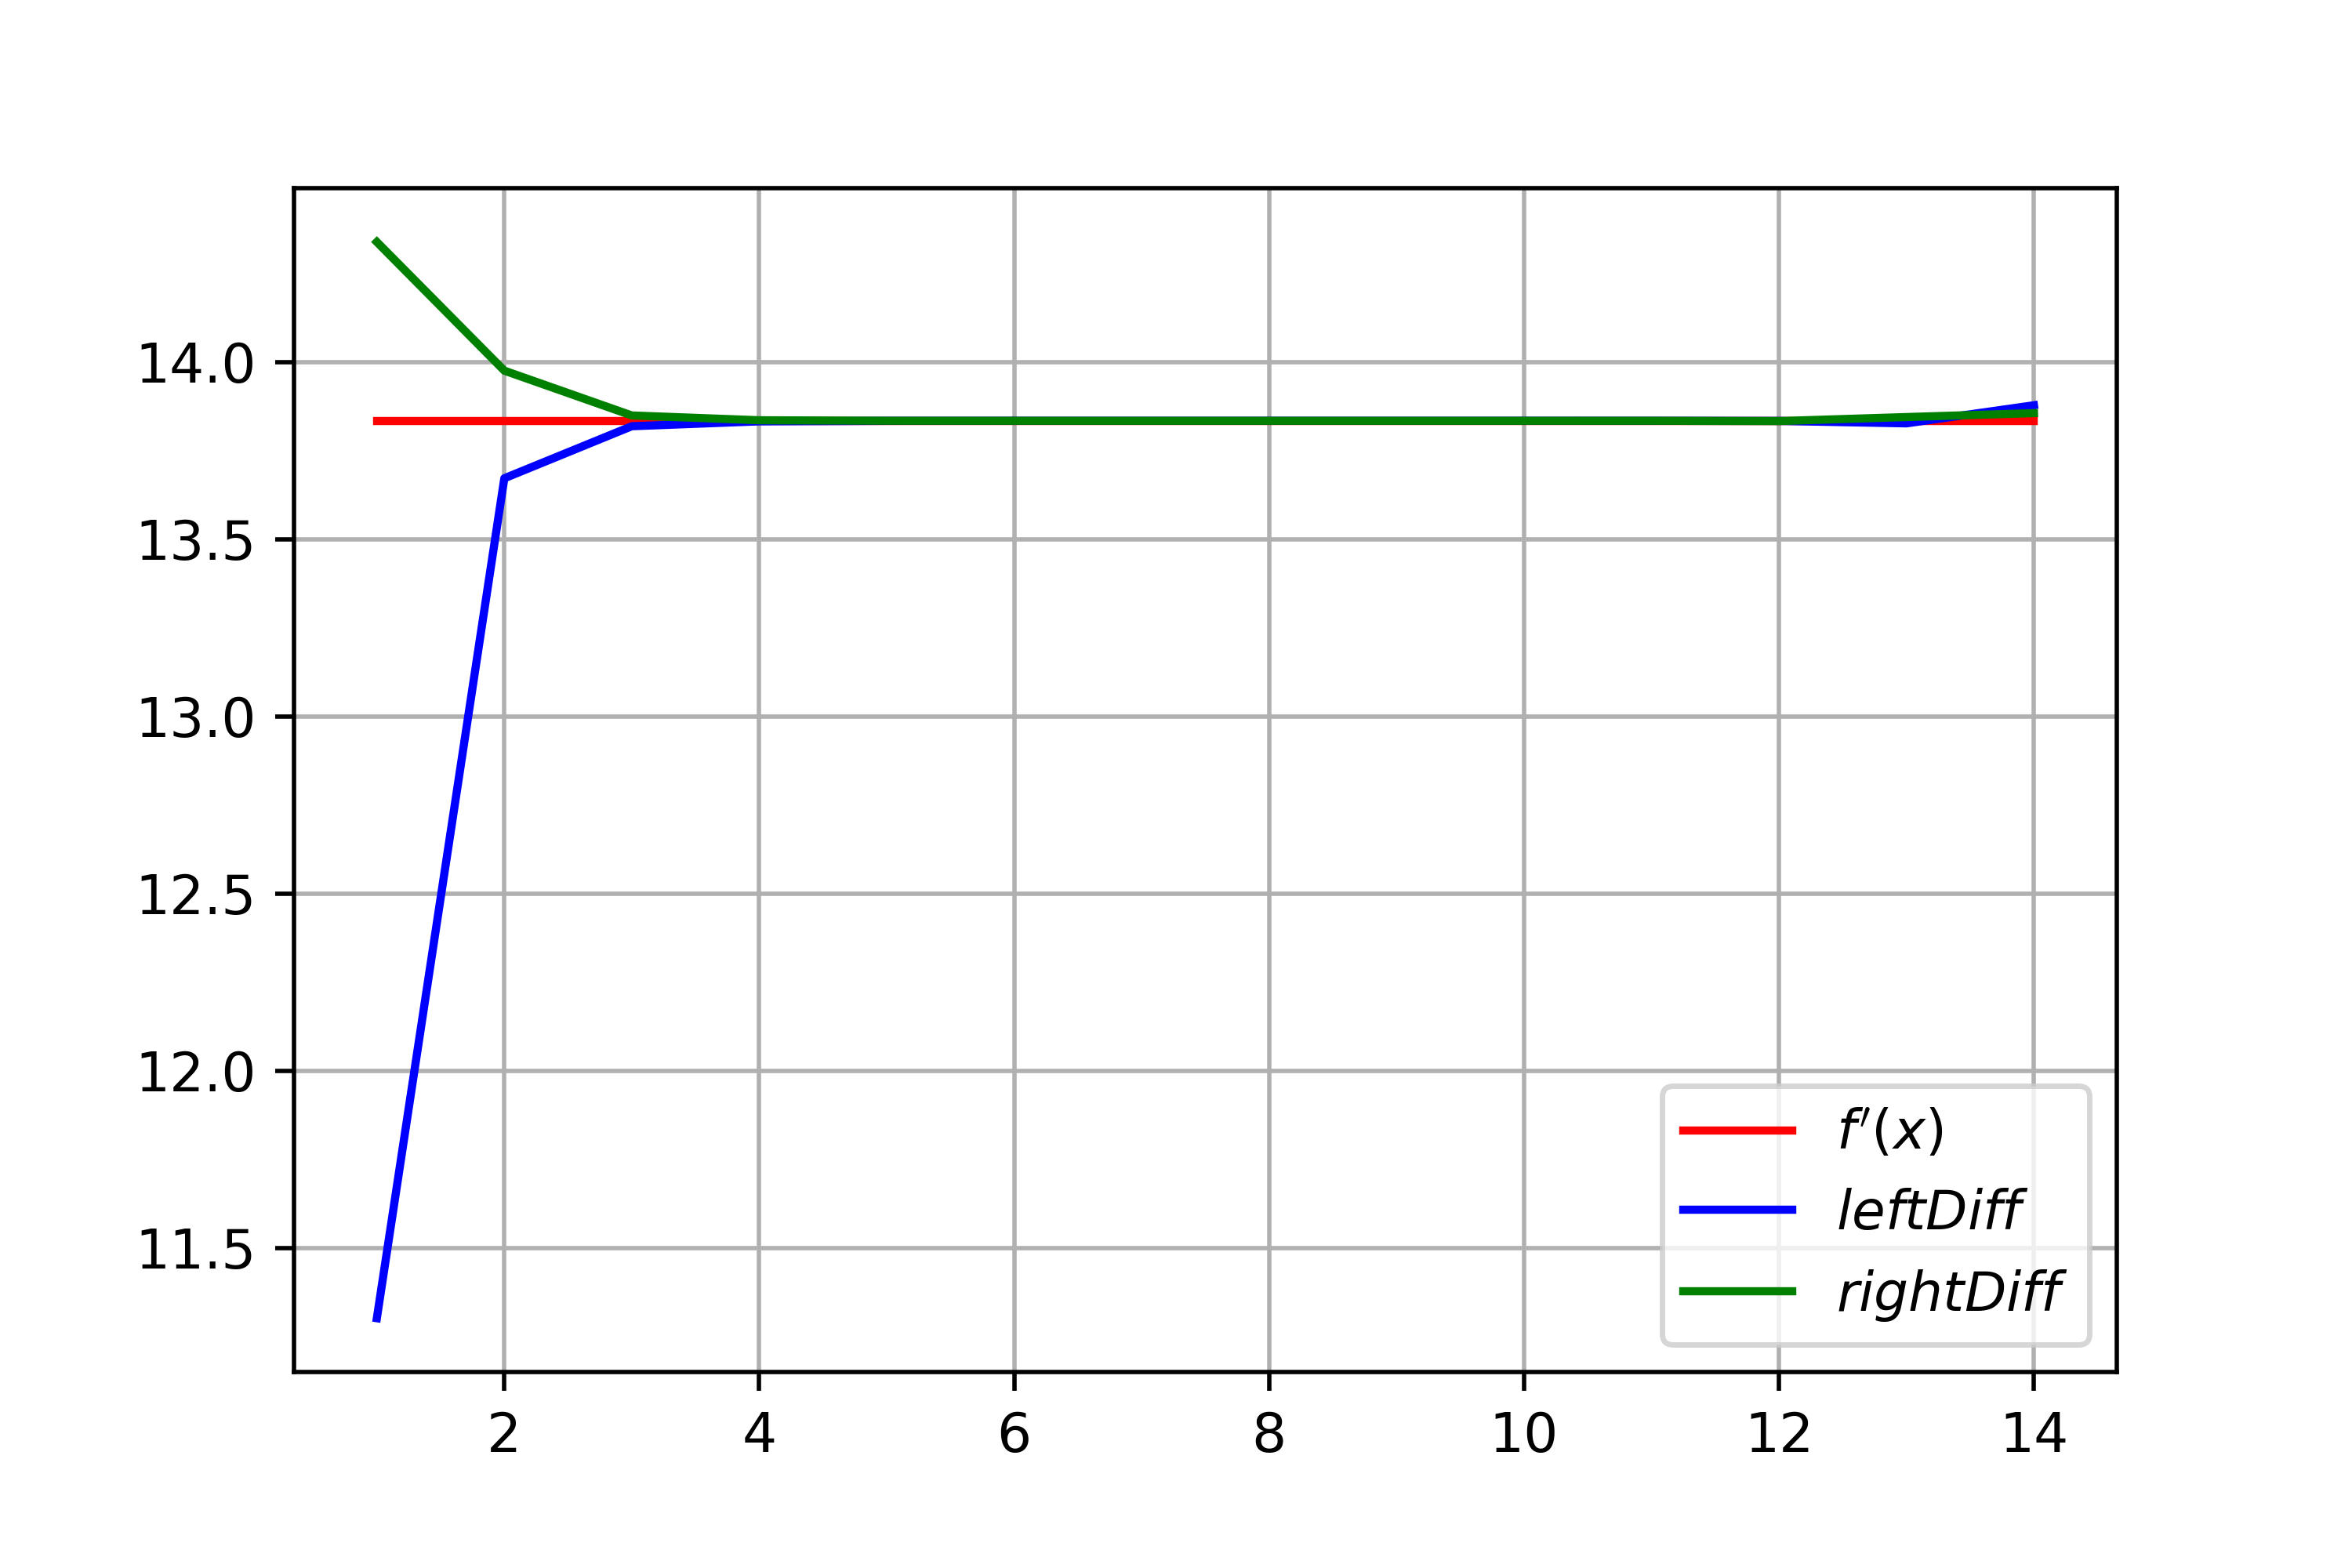
\includegraphics[width=8.5cm]{images/plot_6.1_1st_deriv.png} % первое изображение
	        \caption{Графики производных 1-го порядка, вычисленных с помощью формул левых и правых разностных производных}
	\end{minipage}\hfill
	\begin{minipage}{0.45\textwidth}
		\centering
		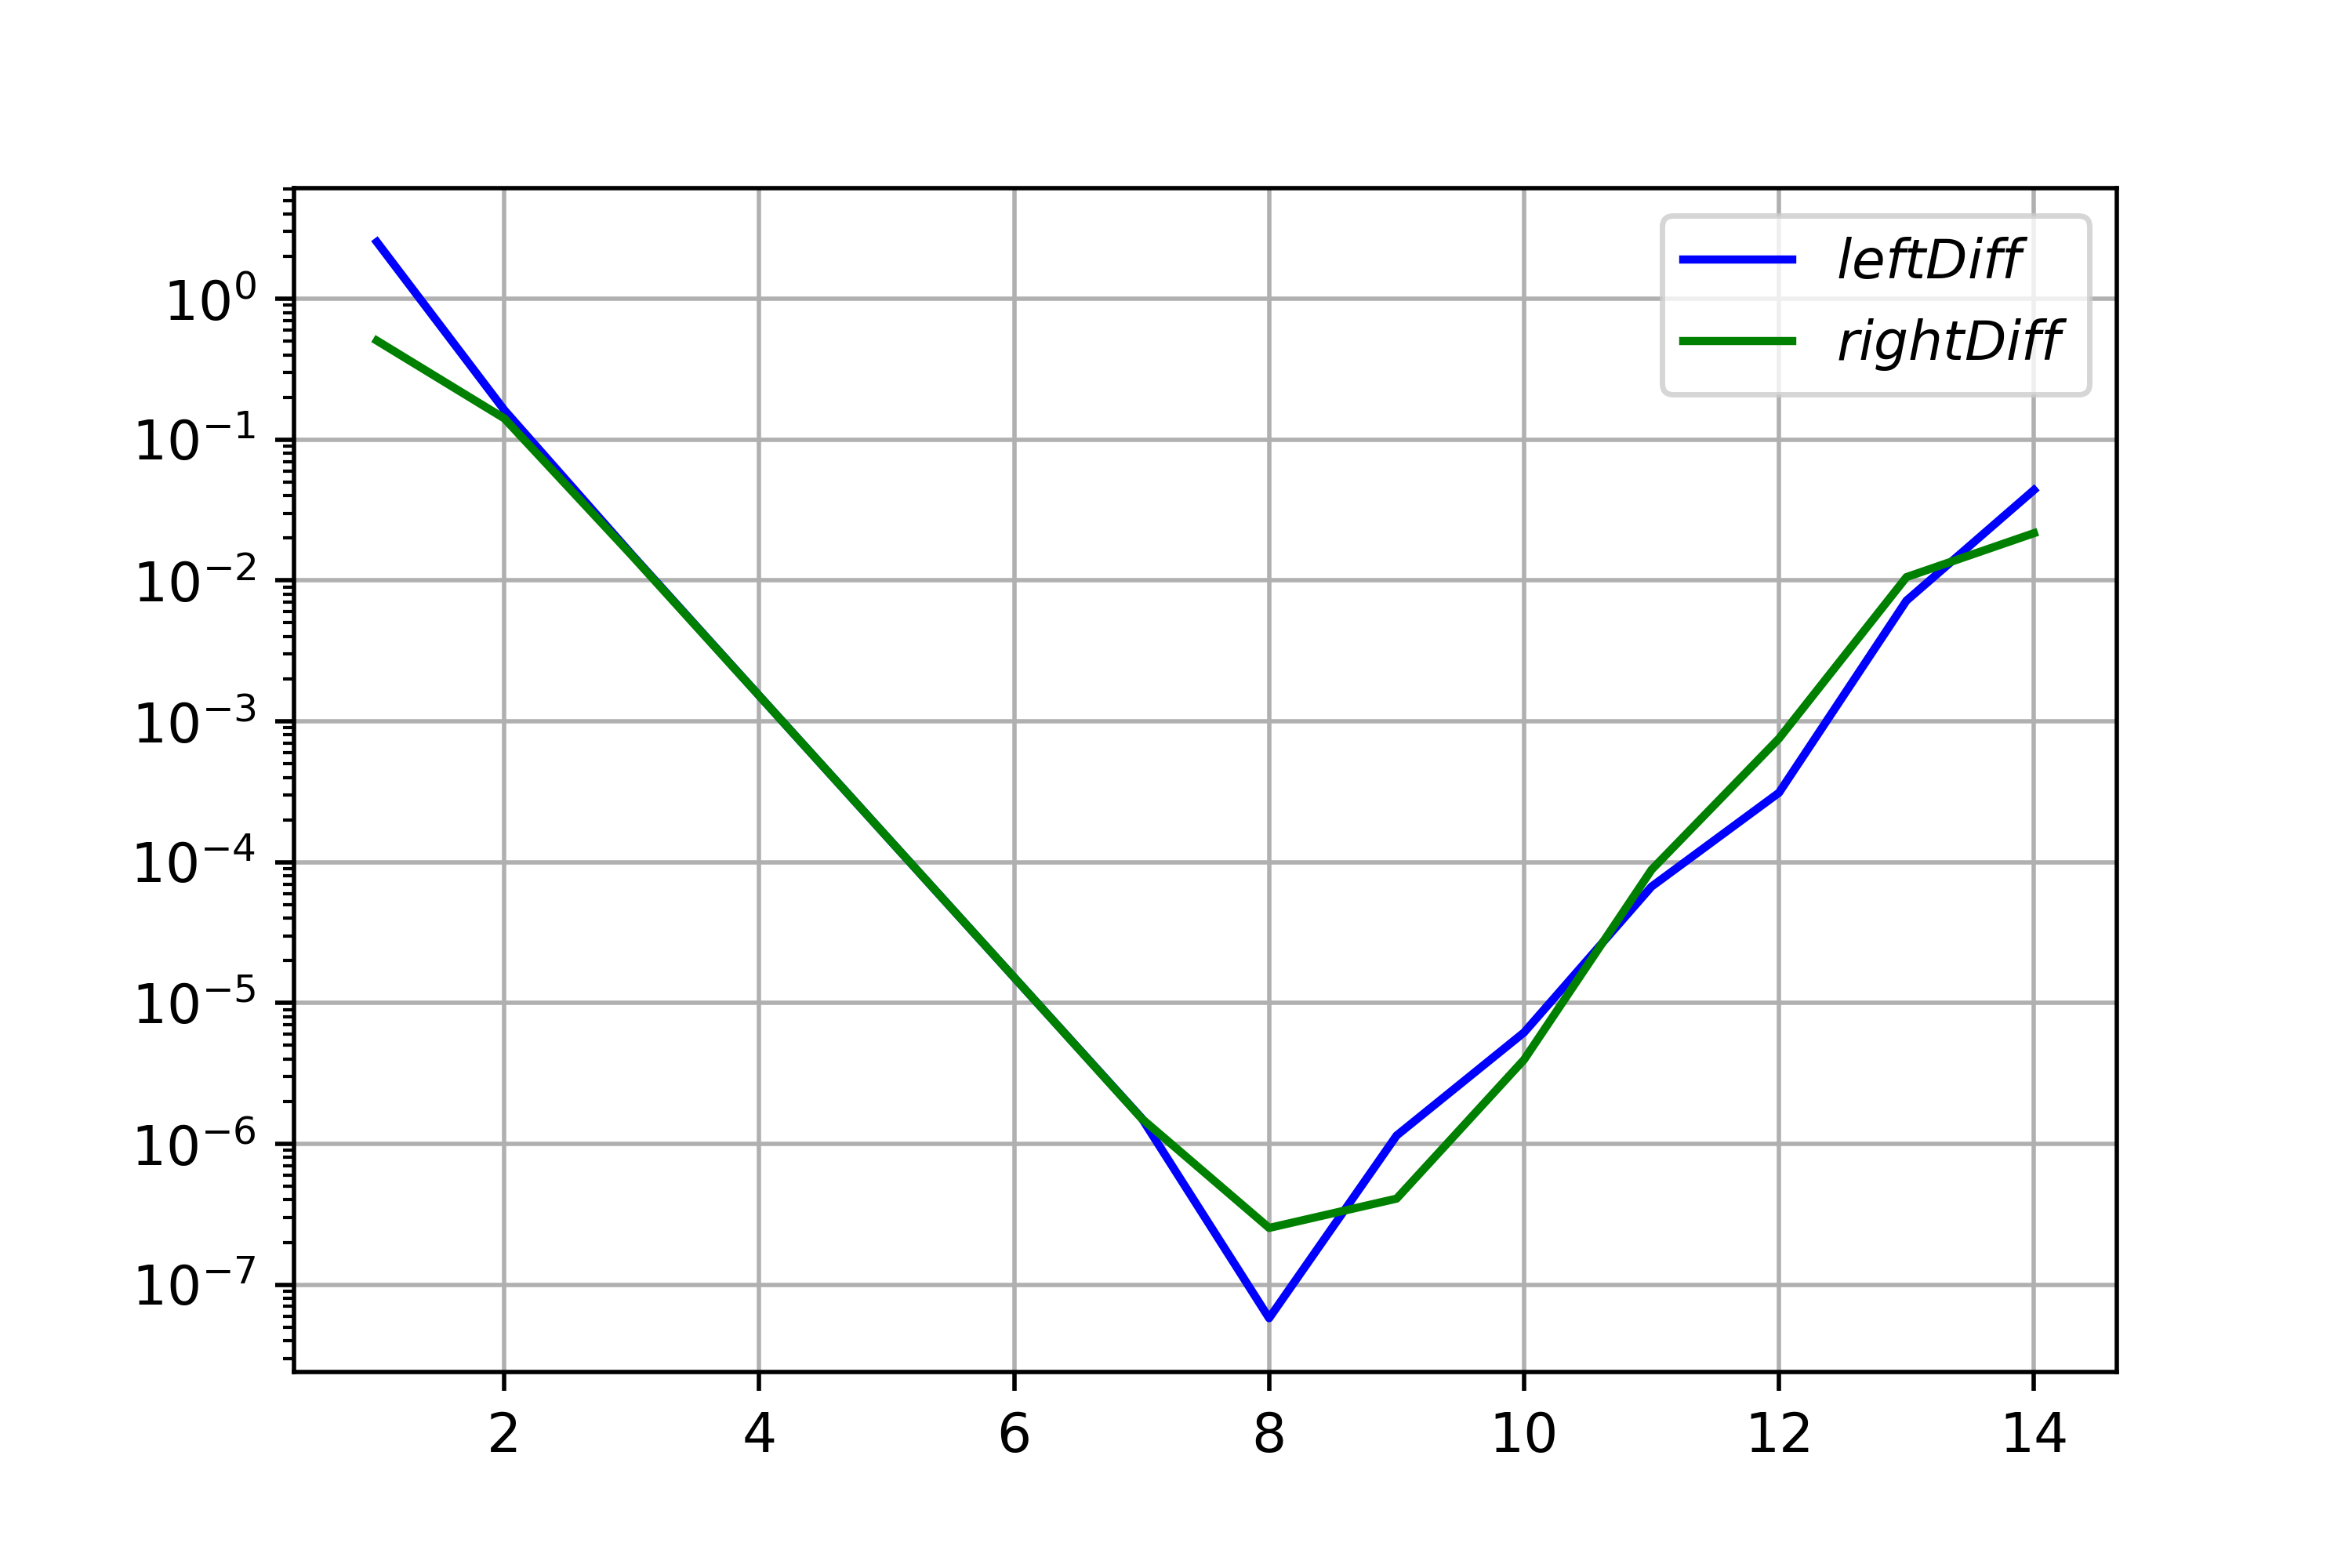
\includegraphics[width=8.5cm]{images/plot_6.1_1st_deriv_err.png} % второе изображение
		\caption{Графики погрешностей вычисления первой производной  по левой и правой формулам разностных производных}
	\end{minipage}
\end{figure}

\begin{figure}[h!]
	\centering                                                                                            
	\begin{minipage}{0.45\textwidth}
	        \centering
	        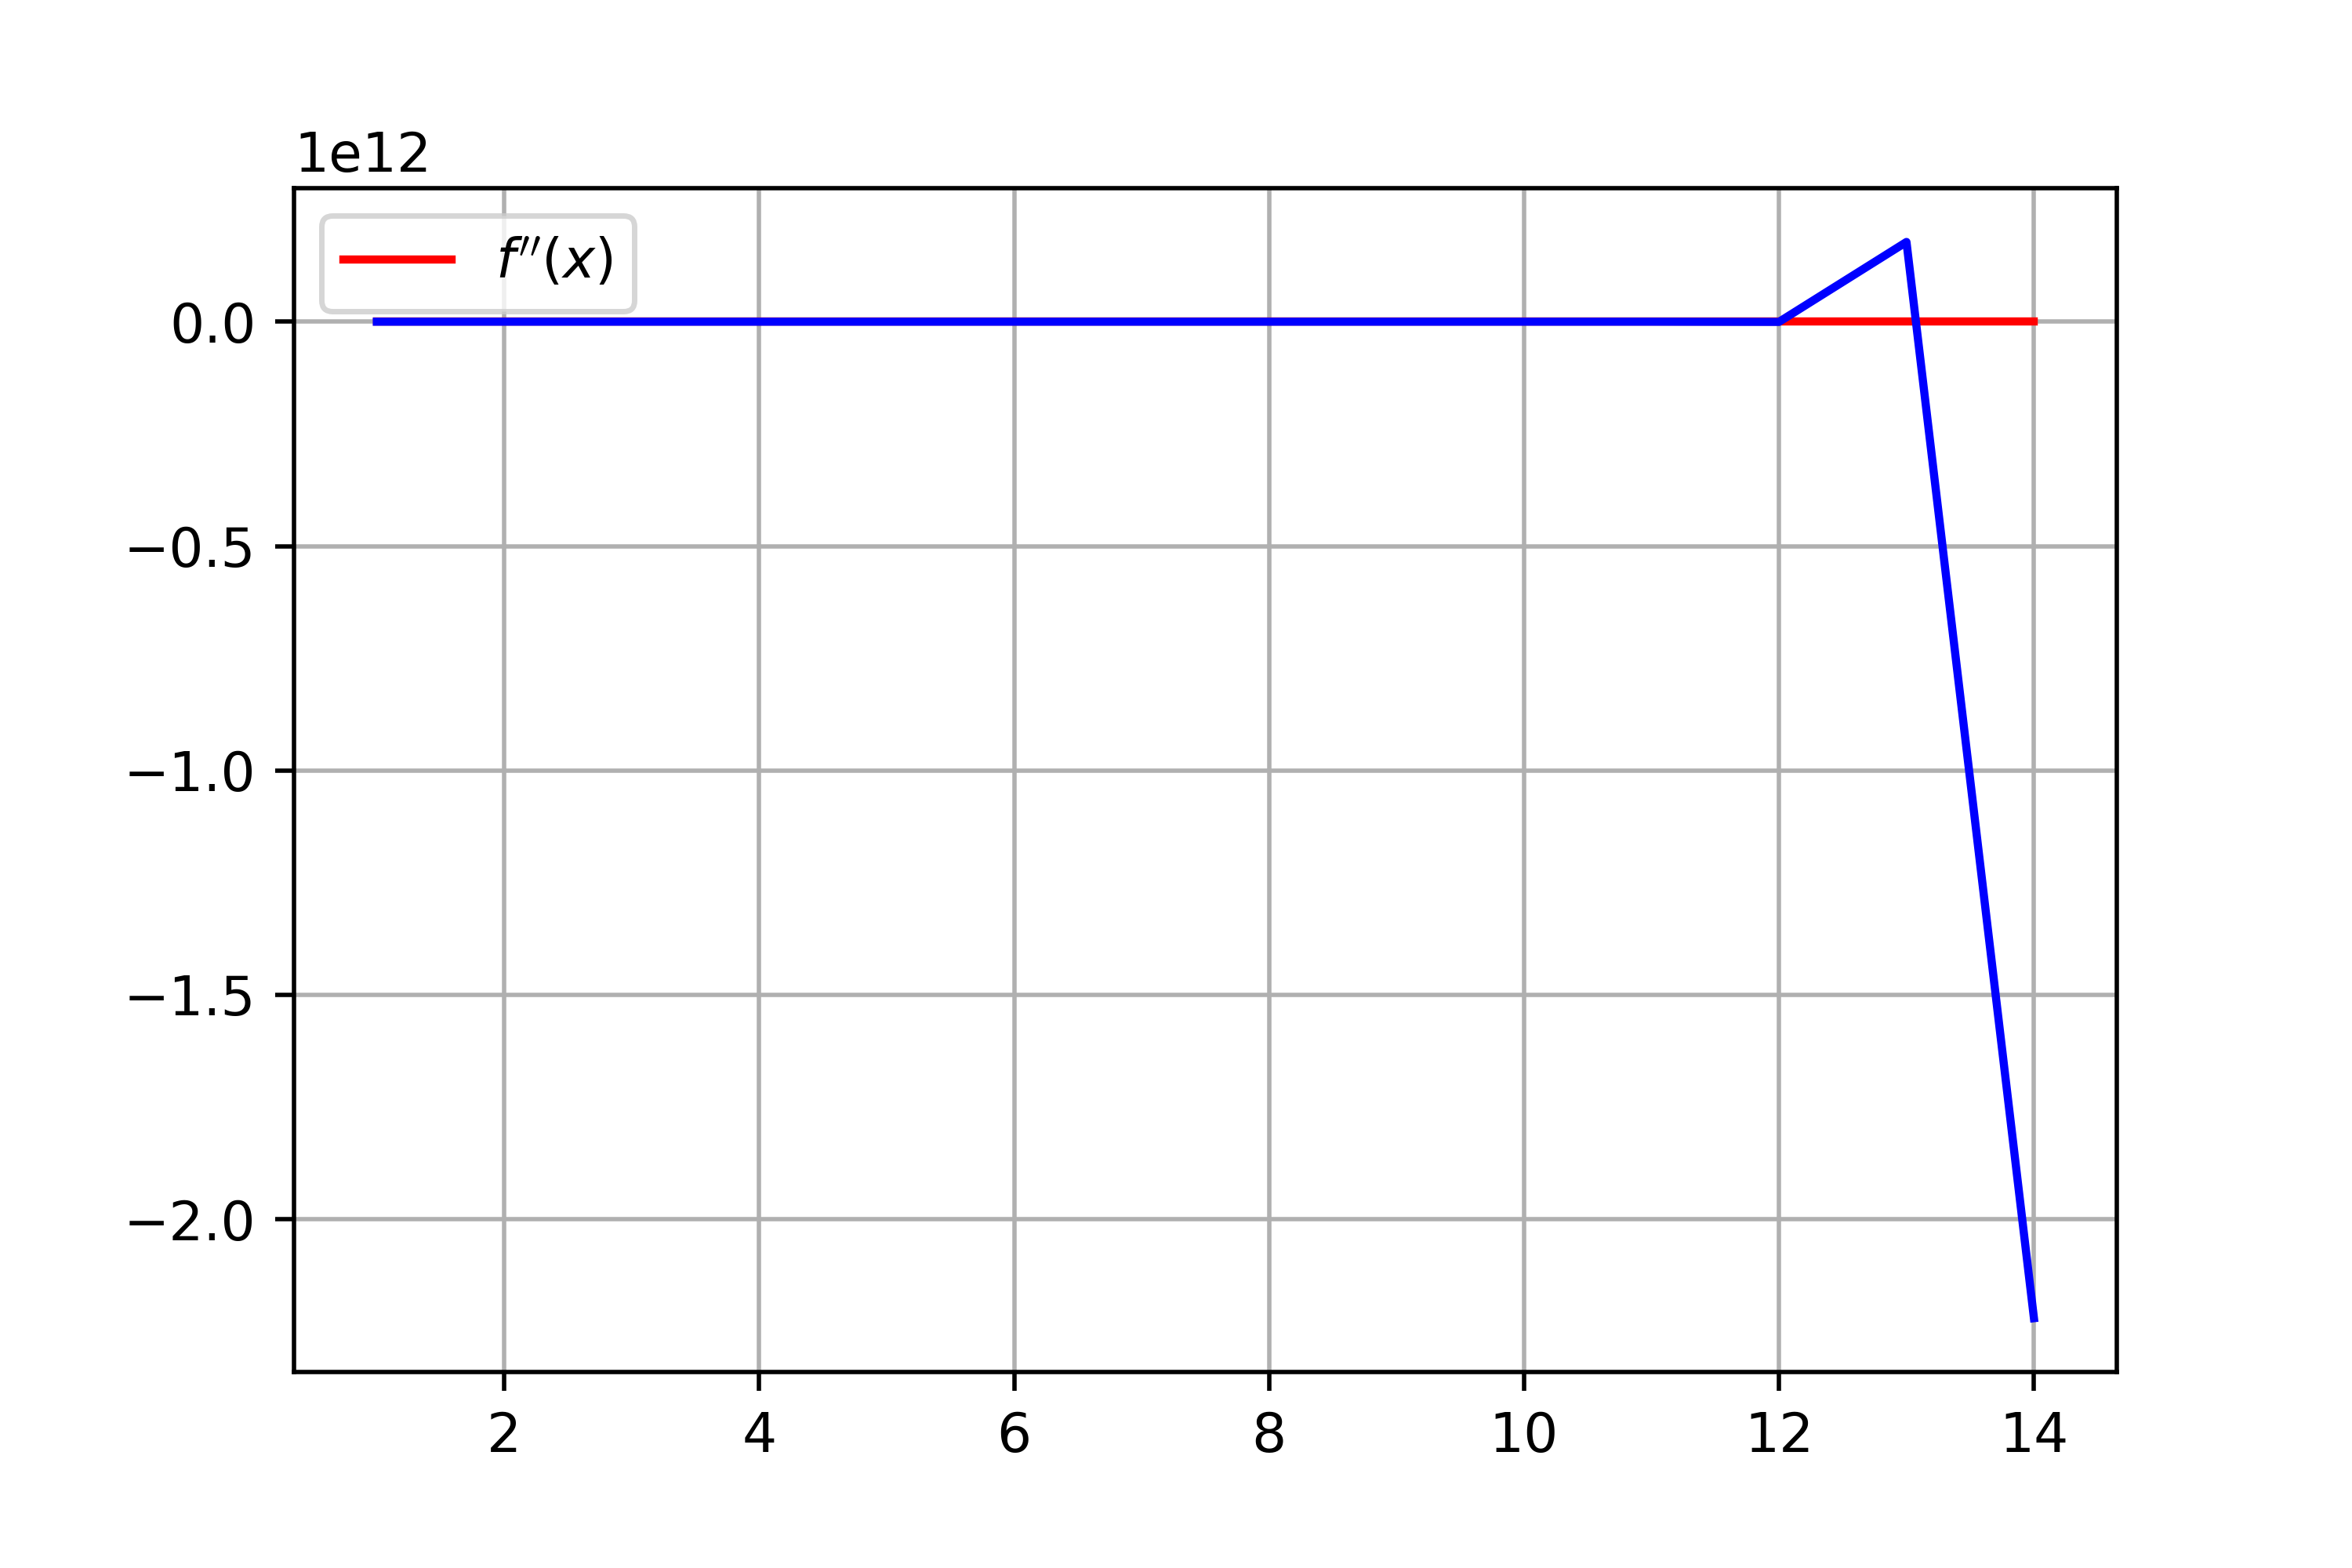
\includegraphics[width=8.5cm]{images/plot_6.1_2nd_deriv.png} % первое изображение
	        \caption{График производной 2-го порядка}
	\end{minipage}\hfill
	\begin{minipage}{0.45\textwidth}
		\centering
		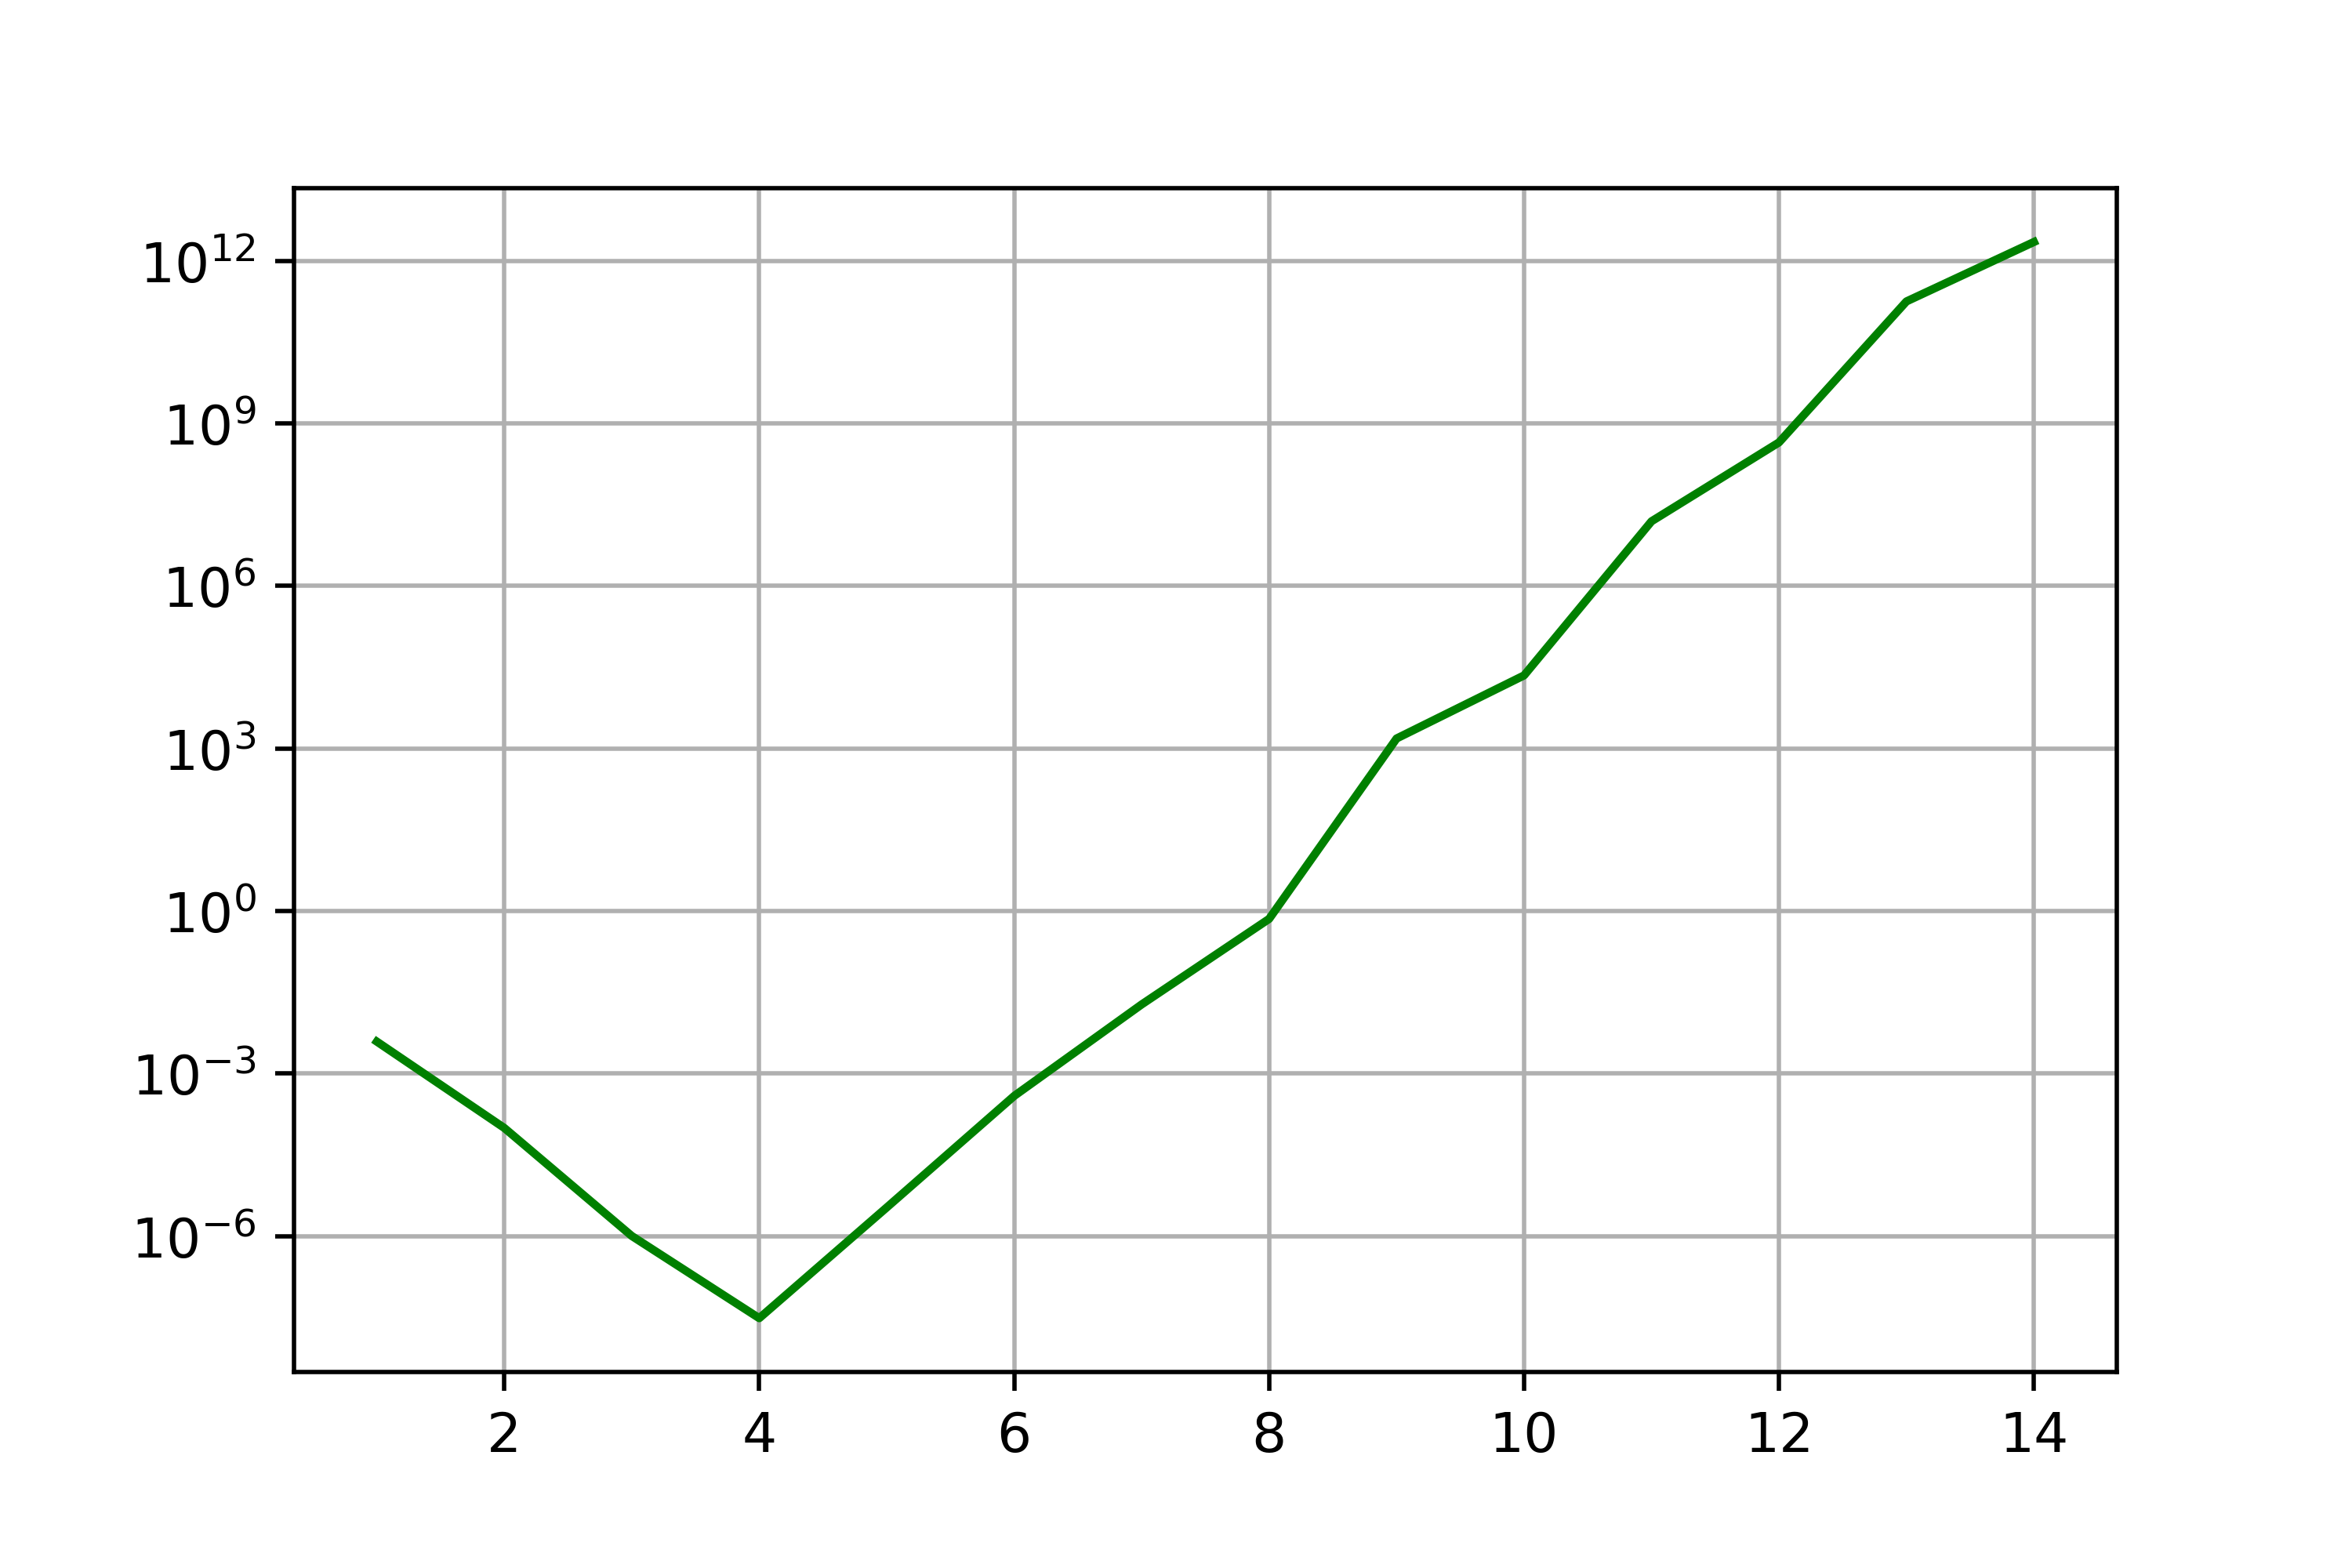
\includegraphics[width=8.5cm]{images/plot_6.1_2nd_deriv_err.png} % второе изображение
		\caption{Погрешность вычисления второй производной}
	\end{minipage}
\end{figure}

\[
\begin{tabular}{| p{3.75cm} | p{3.75cm} | p{3.75cm} | p{3.75cm} |}
	\hline
	$f'(c) = 13.83391227$ & Первый результат \newline при шаге $h = 10^{-1}$ & Наилучший результат \newline при шаге $h = 10^{-8}$ &  Последний результат \newline при шаге $h = 10^{-15}$ \\ \hline
	Формула (1) & $dl_1 = 14.33853900$ \newline $\Delta l_1 = 0.50462672$ &  $dl_1 = 13.83391252$ \newline $\Delta l_1 = 0.00000025$ &  $dl_{15} = 13.76676550$ \newline $\Delta l_{15} = 0.06714676$ \\ \hline
	Формула (2) & $dl_1 = 11.30169535$ \newline $\Delta l_1 = 2.53221691$ & $dl_1 = 13.83391221$ \newline $\Delta l_1 = 0.00000006$ &  $dl_{15} = 13.76676550$ \newline $\Delta l_{15} = 0.06714676$ \\ \hline
	$f''(c) = 30.37231240$ & Первый результат \newline при шаге $h = 10^{-1}$ & Наилучший результат \newline при шаге $h = 10^{-4}$ &  Последний результат \newline при шаге $h = 10^{-15}$ \\ \hline
	Формула (6) & $dl_1 = 30.36843645$ \newline $\Delta l_1 = 0.00387594$ &  $dl_1 = 30.37231237$ \newline $\Delta l_1 = 0.00000003$ &  $dl_{15} = 0.0$ \newline $\Delta l_{15} =30.37231240$ \\ \hline
\end{tabular}
\]

Выведем формулу (6) вычисления второй производной: $f''(x) \approx \dfrac{f(x + h) - 2f(x) + f(x - h)}{h^2}$
Для этого возьмем 3 узла интерполяции и построим по ним многочлен Ньютона 2 степени, а затем дважды продифференцируем его:

\begin{gather*}
	P_2(x) = f_i + \dfrac{\Delta f_i}{h}(x - x_i) + \dfrac{\Delta^2f_i}{2h^2}(x - x_i)(x - x_{i+1}) \\
	P_2'(x) =  \dfrac{\Delta f_i}{h} + \dfrac{\Delta^2f_i}{2h^2}((x - x_i) + (x - x_{i+1})) \\
	P_2''(x) = 2\dfrac{\Delta^2f_i}{2h^2} = \dfrac{f_{i+1} - 2f_i + f_{i-1}}{h^2}
\end{gather*}